%% BioMed_Central_Tex_Template_v1.06
%%                                      %
%  bmc_article.tex            ver: 1.06 %
%                                       %

%%IMPORTANT: do not delete the first line of this template
%%It must be present to enable the BMC Submission system to
%%recognise this template!!

%%% additional documentclass options:
%  [doublespacing]
%  [linenumbers]   - put the line numbers on margins

\documentclass[twocolumn]{bmcart}
%\documentclass{bmcart}

%%% Load packages
%\usepackage{amsthm}
%\RequirePackage{natbib}
%\RequirePackage[authoryear]{natbib}% uncomment this for author-year bibliography
\usepackage{hyperref}
\usepackage[utf8]{inputenc} %unicode support
%\usepackage[applemac]{inputenc} %applemac support if unicode package fails
%\usepackage[latin1]{inputenc} %UNIX support if unicode package fails

\usepackage{graphicx}
\usepackage{minted}
\usemintedstyle{vs}

\usepackage{amsmath,amssymb}
\usepackage{booktabs}


%%%%%%%%%%%%%%%%%%%%%%%%%%%%%%%%%%%%%%%%%%%%%%%%%
%%                                             %%
%%  If you wish to display your graphics for   %%
%%  your own use using includegraphic or       %%
%%  includegraphics, then comment out the      %%
%%  following two lines of code.               %%
%%  NB: These line *must* be included when     %%
%%  submitting to BMC.                         %%
%%  All figure files must be submitted as      %%
%%  separate graphics through the BMC          %%
%%  submission process, not included in the    %%
%%  submitted article.                         %%
%%                                             %%
%%%%%%%%%%%%%%%%%%%%%%%%%%%%%%%%%%%%%%%%%%%%%%%%%


%\def\includegraphic{}
%\def\includegraphics{}

%%% Put your definitions there:
\startlocaldefs
\endlocaldefs

\begin{document}

%%% Start of article front matter
\begin{frontmatter}

\begin{fmbox}
\dochead{Software}

\title{openTSNE: a modular Python library for t-SNE dimensionality reduction and embedding}

%%%%%%%%%%%%%%%%%%%%%%%%%%%%%%%%%%%%%%%%%%%%%%
%%                                          %%
%% Enter the authors here                   %%
%%                                          %%
%% Specify information, if available,       %%
%% in the form:                             %%
%%   <key>={<id1>,<id2>}                    %%
%%   <key>=                                 %%
%% Comment or delete the keys which are     %%
%% not used. Repeat \author command as much %%
%% as required.                             %%
%%                                          %%
%%%%%%%%%%%%%%%%%%%%%%%%%%%%%%%%%%%%%%%%%%%%%%

\author[
   addressref={aff1},                   % id's of addresses, e.g. {aff1,aff2}
   corref={aff1},                       % id of corresponding address, if any
   %noteref={n1},                        % id's of article notes, if any
   email={pavlin.policar@fri.uni-lj.si}   % email address
]{\inits{PGP}\fnm{Pavlin G.} \snm{Poli\v{c}ar}}
\author[
   addressref={aff1,aff2}
]{\inits{MS}\fnm{Martin} \snm{Stra\v{z}ar}}
\author[
   addressref={aff1,aff3}
]{\inits{BZ}\fnm{Bla\v{z}} \snm{Zupan}}

%%%%%%%%%%%%%%%%%%%%%%%%%%%%%%%%%%%%%%%%%%%%%%
%%                                          %%
%% Enter the authors' addresses here        %%
%%                                          %%
%% Repeat \address commands as much as      %%
%% required.                                %%
%%                                          %%
%%%%%%%%%%%%%%%%%%%%%%%%%%%%%%%%%%%%%%%%%%%%%%

\address[id=aff1]{%
  \orgname{Faculty of Computer and Information Science, University of Ljubljana},
  %\street{Ve\v{c}na Pot 113},
  \postcode{SI 1000}
  \city{Ljubljana},
  \cny{Slovenia}
}
\address[id=aff2]{%
  \orgname{Broad Institute of Harvard and MIT},
  %\street{D\"{u}sternbrooker Weg 20},
  \postcode{MA 02142}
  \city{Cambridge},
  \cny{U.S.A.}
}
\address[id=aff3]{%
  \orgname{Department of Molecular and Human Genetics, Baylor College of Medicine},
  %\street{D\"{u}sternbrooker Weg 20},
  \postcode{TX 77030}
  \city{Houston},
  \cny{U.S.A.}
}

%%%%%%%%%%%%%%%%%%%%%%%%%%%%%%%%%%%%%%%%%%%%%%
%%                                          %%
%% Enter short notes here                   %%
%%                                          %%
%% Short notes will be after addresses      %%
%% on first page.                           %%
%%                                          %%
%%%%%%%%%%%%%%%%%%%%%%%%%%%%%%%%%%%%%%%%%%%%%%

%\begin{artnotes}
%\note{Sample of title note}     % note to the article
%\note[id=n1]{Equal contributor} % note, connected to author
%\end{artnotes}

\end{fmbox}% comment this for two column layout

%%%%%%%%%%%%%%%%%%%%%%%%%%%%%%%%%%%%%%%%%%%%%%
%%                                          %%
%% The Abstract begins here                 %%
%%                                          %%
%% Please refer to the Instructions for     %%
%% authors on http://www.biomedcentral.com  %%
%% and include the section headings         %%
%% accordingly for your article type.       %%
%%                                          %%
%%%%%%%%%%%%%%%%%%%%%%%%%%%%%%%%%%%%%%%%%%%%%%

\begin{abstractbox}

\begin{abstract}
Point-based visualisations of large, multi-dimensional data from
molecular biology can reveal meaningful clusters. One of the
most popular techniques to construct such visualisations is t-distributed
stochastic neighbor embedding (t-SNE), for which a number of extensions have
recently been proposed to address issues of scalability and the quality of the resulting
visualisations. We introduce openTSNE, a modular Python library that implements
the core t-SNE algorithm and its extensions. The library is orders of magnitude
faster than existing popular implementations, including those from
scikit-learn. Unique to openTSNE is also the mapping of new data to existing embeddings, which
can surprisingly assist in solving batch effects.
\end{abstract}

%%%%%%%%%%%%%%%%%%%%%%%%%%%%%%%%%%%%%%%%%%%%%%
%%                                          %%
%% The keywords begin here                  %%
%%                                          %%
%% Put each keyword in separate \kwd{}.     %%
%%                                          %%
%%%%%%%%%%%%%%%%%%%%%%%%%%%%%%%%%%%%%%%%%%%%%%

\begin{keyword}
\kwd{sample}
\kwd{article}
\kwd{author}
\end{keyword}

% MSC classifications codes, if any
%\begin{keyword}[class=AMS]
%\kwd[Primary ]{}
%\kwd{}
%\kwd[; secondary ]{}
%\end{keyword}

\end{abstractbox}
%
%\end{fmbox}% uncomment this for twcolumn layout

\end{frontmatter}

%%%%%%%%%%%%%%%%%%%%%%%%%%%%%%%%%%%%%%%%%%%%%%
%%                                          %%
%% The Main Body begins here                %%
%%                                          %%
%% Please refer to the instructions for     %%
%% authors on:                              %%
%% http://www.biomedcentral.com/info/authors%%
%% and include the section headings         %%
%% accordingly for your article type.       %%
%%                                          %%
%% See the Results and Discussion section   %%
%% for details on how to create sub-sections%%
%%                                          %%
%% use \cite{...} to cite references        %%
%%  \cite{koon} and                         %%
%%  \cite{oreg,khar,zvai,xjon,schn,pond}    %%
%%  \nocite{smith,marg,hunn,advi,koha,mouse}%%
%%                                          %%
%%%%%%%%%%%%%%%%%%%%%%%%%%%%%%%%%%%%%%%%%%%%%%

%%%%%%%%%%%%%%%%%%%%%%%%% start of article main body
% <put your article body there>

%%%%%%%%%%%%%%%%
%% Background %%
%%
\section*{Background}

%We implement t-SNE~\cite{maaten2008visualizing}. We include a set of recommendations and tricks from Kobak and Berens~\cite{kobak2019art} as well as incerasing the learning rate as recommended by Belkina \textit{et al.}~\cite{belkina2019automated}. Also support using variable degrees of freedom by Kobak \textit{et al.}~\cite{kobak2019heavy}.
%
%Two approximation schemes, one based on Barnes-Hut~\cite{van2014accelerating} and one on the interpolation-based approach~\cite{linderman2019fast}.
%
%UMAP~\cite{2018arXivUMAP}, whether or not it better preserves global structure or not is in question~\cite{kobak2019umap}.


%% TODO: START FROM FIRST PAPER

The abundance of high-dimensional data sets in molecular biology calls for
techniques for dimensionality reduction, and in particular for methods that can
help in the construction of data visualizations. Popular approaches for
dimensionality reduction include principal component analysis, multidimensional
scaling, and uniform manifold approximation and projections~\cite{2018arXivUMAP}. Among
these, t-distributed stochastic neighbor embedding
(t-SNE)~\cite{maaten2008visualizing} lately received much attention as it can
address high volumes of data and reveal meaningful clustering structure. Most
of the recent reports on single-cell gene expression data start with an
overview of the cell landscape, where t-SNE embeds high-dimensional expression
profiles into a two-dimensional space~\cite{macosko2015highly,cao2019single,tasic2018shared}.
Fig.~\ref{fig:tsne}.a presents an example of one such embedding.

Despite its utility, t-SNE has been criticized for poor scalability
when addressing large data sets, lack of global organization \em t-SNE
focuses on local clusters that are arbitrarily scattered in the
low-dimensional space \em and absence of theoretically-founded implementations to
map new data into existing embeddings~\cite{ding2018interpretable,becht2019dimensionality}. Most of these shortcomings, have
recently been addressed.
\cite{fi_tsne} sped-up the method through an interpolation-based
approximation, reducing the time complexity to be merely linear dependent on the number of samples. \cite{art_of_using_tsne} proposed
several techniques to improve global positioning, including estimating similarities with a mixture of
Gaussian kernels. While no current popular
software library supports mapping of new data into reference embedding,
\cite{parametric_tsne} proposed a related approach
using neural networks.

%% TODO: END FROM FIRST PAPER


\begin{figure*}[htbp]
  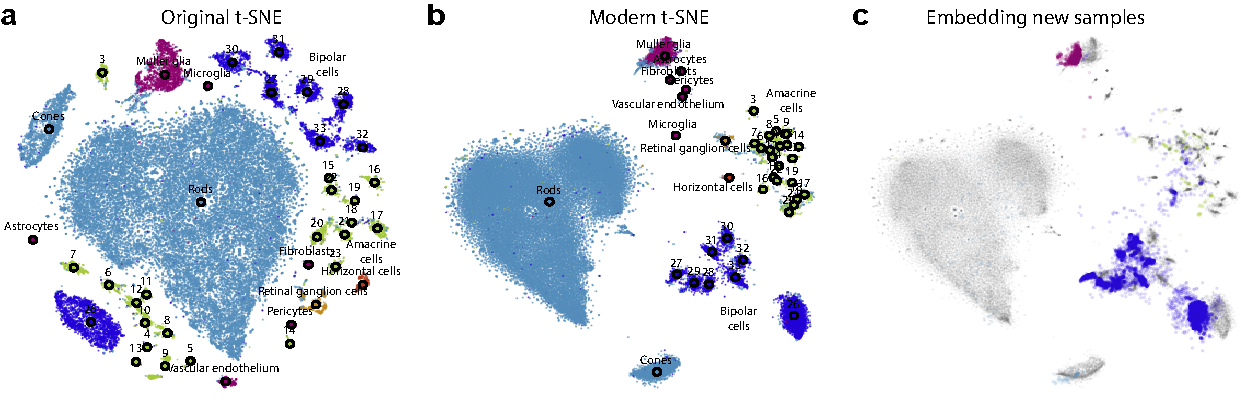
\includegraphics[width=\textwidth]{macosko2015}
  \caption{\label{fig:macosko}}
\end{figure*}

\section*{Results}


We introduce openTSNE, a comprehensive Python library that
implements t-SNE and all its recently proposed extensions. The library is
compatible with the Python data science ecosystem (e.g., {\tt numpy}, {\tt
sklearn}, {\tt scanpy}). Its modular design encourages extendibility and
experimentation with various settings and changes in the analysis pipeline.


\begin{figure*}[htbp]
  \includegraphics[width=\textwidth]{tasic2018}
  \caption{\label{fig:tasic}We use openTSNE to create four different visualizations of the Tasic \textit{et al.}~\cite{tasic2018shared} data set containing 21,874 single-cells originating from the mouse neocortex. Cluster annotations and colors are taken from the original publication. Warm colors correspond to excitatory neurons, cool colors correspond to inhibitory neurons, and gray/brown colors correspond to non-neuronal cells. The standard t-SNE \textbf{(a)} emphasizes local structure, while increasing perplexity \textbf{(b)} results in a more meaningful layout of the clusters. We can also combine the two perplexities by using a multiscale kernel affinity model \textbf{(c)} and obtain a good trade-off between global and local structure. Alternatively, we can inspect more fine-grained structure and reveal smaller clusters by using a more heavy-tailed kernel \textbf{(d)}.}
\end{figure*}

The following code is used to generate Fig.~\ref{fig:tasic}
\begin{minted}[fontsize=\footnotesize]{python}
# Perplexity 30 (standard t-SNE)
perp_30 = openTSNE.TSNE(
    perplexity=30, metric="cosine"
).fit(X)

# Perplexity 500 (emphasise global structure)
perp_500 = openTSNE.TSNE(
    perplexity=500, metric="cosine"
).fit(X)

# Multiscale kernel with perplexities 30,500
affinities = openTSNE.affinity.Multiscale(
    X, perplexities=[30, 500], metric="cosine"
)
init = openTSNE.initialization.pca(X)
ms = openTSNE.TSNEEmbedding(init, affinities)
ms = ms.optimize(n_iter=250, exaggeration=12)
ms = ms.optimize(n_iter=250, exaggeration=1)

# Expose finer structure using smaller dof
perp_30 = openTSNE.TSNE(
    perplexity=30, metric="cosine", dof=0.6
).fit(X)
\end{minted}


\begin{figure*}[htbp]
  \includegraphics[width=\textwidth]{cao2019}
  \caption{\label{fig:cao}The data set from Cao \textit{et al.}~\cite{cao2019single} contains expression profiles from 2,058,652 single cells. The data were collected from mice embryos at different developmental time-points at daily intervals after 9.5 to 13.5 days. The exaggeration parameter can be used to highlight the global organization of the clusters and enforce cluster compactness. \textbf{(a)} shows the data is comprised of two main components -- the neural tube and mesenchymal cells -- as well as several other smaller clusters. Additionally, the colors indicate developmental progression with red indicating least-developed cells and blue indicating most developed cells. The overall developmental trajectory is most apparent with higher levels of exaggeration, showing red cells slowly transitioning into blue cells. Progressively easing the exaggeration factor uncovers finer clusters within the larger groups as shown in \textbf{(b)} with exaggeration 2 and subsequently in \textbf{(c)}, where we show the standard t-SNE with no exaggeration. 32,011 putative doublets are excluded from the visualizations.}
\end{figure*}


The following code is used to generate Fig.~\ref{fig:cao}
\begin{minted}[fontsize=\footnotesize]{python}
indices = np.random.permutation(list(range(x.shape[0])))
reverse = np.argsort(indices)
# Split the data into a sample/remainder sets
x_sample, x_rest = x[indices[:25000]], x[indices[25000:]]
y_sample, y_rest = y[indices[:25000]], y[indices[25000:]]
# Create an initial embedding using a subset of the data
sample_embedding = openTSNE.TSNE(
    initialization="spectral",
    perplexity=500,
    metric="cosine",
).fit(x_sample)
# Position the remainder of the points to their nearest
# neighbor in the sample embedding
rest_init = sample_embedding.prepare_partial(x_rest, k=1)
init_full = np.vstack(
    [sample_embedding, rest_init]
)[reverse]
init_full = openTSNE.initialization.rescale(init_full)
# Calculate the affinity model using all the data points
affinities = openTSNE.affinity.PerplexityBasedNN(
    x, perplexity=30, metric="cosine"
)

embedding = openTSNE.TSNEEmbedding(
    init_full, affinities
%)
exag12 = embedding.optimize(n_iter=500, exaggeration=12)
exag4 = exag12.optimize(n_iter=500, exaggeration=4)
exag2 = exag4.optimize(n_iter=500, exaggeration=2)
exag1 = exag2.optimize(n_iter=500, exaggeration=1)
\end{minted}


\begin{figure*}[htbp]
  \includegraphics[width=\textwidth]{transform_hochgerner}
  \caption{\label{fig:transform}openTSNE enables the user to embed new samples into an existing, reference embedding. We construct a t-SNE embedding for the data from Hochgerner \textit{et al.}~\cite{hochgerner2018conserved} containing 24,185 developing, single cells from the mouse hippocampus. The data contains different types of neurons, supporting glia, and other vascular cells (upper left). Cell annotations are taken from the original publications. The colors correspond to Fig.~\ref{fig:tasic}. We then embed new, hippocampal cells collected by Harris \textit{et al.}~\cite{harris2018classes} using the previous embedding as a reference. In their study, Harris \textit{et al.} collected 6,971 single-cells and focused on identifying different types of inhibitory neurons. However, almost half of the collected cells are not neurons and were left uncharacterized. Inspecting where these cells are embedded in the reference embedding (bottom left) reveals that in addition to inhibitory neurons, the data contains a number of supporting glia as well as a small population of endothelial cells. We can verify the accuracy of our approach by inspecting marker genes for the major cell types in the reference (top row) and embedded samples (bottom row).}
\end{figure*}


The following code is used to generate Fig.~\ref{fig:transform}
\begin{minted}[fontsize=\footnotesize]{python}
# Assuming we have prepared a reference embedding and
# assuming we have aligned new_X to the reference X matrix
new_embedding = reference_embedding.transform(new_X)
\end{minted}

We want to mention that this works for mitigating batch effects in our earlier work~\cite{policar2019embedding}.


\begin{figure*}[htbp]
  \includegraphics[width=\textwidth]{benchmarks}
  \caption{\label{fig:benchmarks}We benchmark openTSNE against three popular open-source implementations including scikit-learn~\cite{pedregosa2011scikit}, MulticoreTSNE~\cite{Ulyanov2016}, and FIt-SNE~\cite{linderman2019fast}. Benchmarks were run on a consumer-grade Intel Core i7-7700HQ processor found in laptop computers, and on a server-grade Intel Xeon E5-2650. To generate benchmark data sets of different sizes, we subsampled data from the 10X Genomics 1.3 million mouse brain data set five times, resulting in five different data sets for each size. In total, each implementation was run on 30 different data sets. Notice that openTSNE scales similarly to FIt-SNE, as they both use the same interpolation-based approximation scheme, while scikit-learn and MulticoreTSNE utilize the Barnes-Hut approximation.}
\end{figure*}

\section*{Discussion}
Text for this section \ldots

\section*{Conclusion}
Text for this section \ldots

\section*{Methods}

% approach name in bold, reference, description of the approach and why is
% it useful. focus on theory and math.

\subsection*{t-SNE}
%% TODO: Reword this entirely

Local, non-linear dimensionality reduction by t-SNE is performed as follows.
Given a multi-dimensional data set $\mathbf{X} = \left \{ \mathbf{x}_1,
\mathbf{x}_2, \dots, \mathbf{x}_N \right \} \in \mathbb{R}^D$ where $N$ is the
number of data points in the reference data set, t-SNE aims to find a low
dimensional embedding $\mathbf{Y} = \left \{ \mathbf{y}_1, \mathbf{y}_2, \dots,
\mathbf{y}_N \right \} \in \mathbb{R}^d$ where $d \ll D$, such that if points
$\mathbf{x}_i$ and $\mathbf{x}_j$ are close in the multi-dimensional space,
their corresponding embeddings $\mathbf{y}_i$ and $\mathbf{y}_j$ are also
close. Since t-SNE is primarily used as a visualization tool, $d$ is typically
set to two. The similarity between two data points in t-SNE is defined as:

\begin{equation}
p_{j \mid i} = \frac{\exp \left ( -\frac{1}{2} \mathcal{D}(\mathbf{x}_i, \mathbf{x}_j ) / \sigma_i^2 \right )}
{\sum_{k \neq i } \exp \left ( -\frac{1}{2} \mathcal{D}(\mathbf{x}_i, \mathbf{x}_k ) / \sigma_i^2 \right )}, \quad p_{i \mid i} = 0
\label{eq:gaussian_kernel}
\end{equation}

\noindent where $\mathcal{D}$ is a distance measure. This is then symmetrized to

\begin{equation}
p_{ij} = \frac{p_{j \mid i} + p_{i \mid j}}{2N}.
\label{eq:symmetrize}
\end{equation}

The bandwidth of each Gaussian kernel $\sigma_i$ is selected such that the
perplexity of the distribution matches a user-specified parameter value

\begin{equation}
\text{Perplexity} = 2^{H(P_i)}
\end{equation}

\noindent where $H(P_i)$ is the Shannon entropy of $P_i$,

\begin{equation}
H(P_i) = -\sum_i p_{j \mid i} \log_2 (p_{j \mid i}).
\end{equation}

\noindent Different bandwidths $\sigma_i$ enable t-SNE to adapt to the varying
density of the data in the multi-dimensional space.

The similarity between points $\mathbf{y}_i$ and $\mathbf{y}_j$ in the
embedding space is defined using the $t$-distribution with one degree of
freedom

\begin{equation}
q_{ij} = \frac{\left ( 1 + || \mathbf{y}_i - \mathbf{y}_j ||^2 \right )^{-1}}
{\sum_{k \neq l}\left ( 1 + || \mathbf{y}_k - \mathbf{y}_l ||^2 \right )^{-1}},
\quad q_{ii} = 0.
\label{eq:cauchy_kernel}
\end{equation}

The t-SNE method finds an embedding $\mathbf{Y}$ that minimizes the
Kullback-Leibler (KL) divergence between $\mathbf{P}$ and $\mathbf{Q}$,

\begin{equation}
C = \text{KL}(\mathbf{P} \mid \mid \mathbf{Q}) = \sum_{ij} p_{ij} \log \frac{p_{ij}}{q_{ij}}.
\label{eq:kl_divergence}
\end{equation}

It is then easy to show that the corresponding gradient takes on the form
\begin{equation}
\frac{\partial C}{\partial \mathbf{y}_i} = 4 \sum_{j \neq i} \left ( p_{ij} - q_{ij} \right ) \left ( \mathbf{y}_i - \mathbf{y}_j \right ) \left ( 1 + || \mathbf{y}_i - \mathbf{y}_j || ^2 \right )^{-1}.
\label{eq:tsne_gradient}
\end{equation}

Optimization is performed using batch gradient descent with the delta-bar-delta update rule for increased convergence speed~\cite{jacobs1988increased}. Originally, t-SNE was run for 1000 iterations consisting of two phases. In the first \textit{early exaggeration} phase, the attractive forces between data points is increased by a factor $\rho=12$ so that points can move throughout the embedding uninhibited by repulsive forces. Then the remaining 750 iterations are run with $\rho=1$, which reverts the attractive forces to their original values.

Belkina \textit{et al.} later found that the number of iterations can saftely be decreased to 750 iterations by increasing the learning rate to $\eta=N/12$ instead of the default and somewhat arbitrarily set $\eta=200$~\cite{belkina2019automated}. A welcome side effect of this reduction is also faster runtime.

\subsection*{Efficient Implementation}
A direct evaluation of t-SNE gradients requires $\mathcal{O}(N^2)$ operations, which makes its application impractical to any reasonably-sized data set and beckons for the development of efficient approximation schemes. Van der Maaten observed that the t-SNE gradient may be reformulated in terms of a N-body problem where data points may be interpreted as particles which attract and repel each other~\cite{van2014accelerating}. The gradient may be rewritten as
\begin{equation}
\frac{\partial C}{\partial \mathbf{y}_i} = 4 \left [ \sum_{j \neq i} p_{ij} q_{ij} Z \left ( \mathbf{y}_i - \mathbf{y}_j \right ) -\sum_{j \neq i} q_{ij}^2 Z \left ( \mathbf{y}_i - \mathbf{y}_j \right ) \right ], \label{eq:grad_attr_rep}
\end{equation}
where $Z = \sum_{k \neq l}\left ( 1 + || \mathbf{y}_k - \mathbf{y}_l ||^2 \right )^{-1}$. The two terms may be viewed as the attractive and repulsive forces between particles, respectively. Each term lends itself to efficient approximations, which enable us to greatly reduce the time complexity of t-SNE.

\subsubsection*{Attractive Forces}

Van der Maaten observed that since $p_{ij}$ is calculated in the high-dimensional space using a Gaussian kernel, and that the bandwidth is selected such that only a fixed number of closest neighbors (determined by the perplexity parameter) will contribute to the attractive forces of a given point due to the exponential decay of the Gaussian kernel. Therefore it is sufficient to calculate the attractive forces only over a relatively small number of nearest neighbors instead of all $N$ points. By utilizing tree-based nearest-neighbor search methods, the time complexity is thus reduced to $\mathcal{O}(N \log N)$. Linderman \textit{et al.} further realised that, qualitatively, embeddings are visually virtually indistinguishable when using only \textit{approximate} nearest neighbors, further reducing time complexity to $\mathcal{O}(N)$~\cite{linderman2019fast}.

\subsubsection*{Repulsive Forces}

Examining the second term of Eqn.~(\ref{eq:grad_attr_rep}) we notice that each point indiscriminately exerts a repulsive force on all other points. Van der Maaten proposed an approach based on N-body simulations and used a space-partitioning Barnes-Hut tree approach to approximate the interaction between data points. Briefly, the approach splits the space into quadrants (in the 2D case) and if a given point is far enough away from a quadrant, the points in that quadrant are summarized by a single center of mass. This reduces the time complexity from $\mathcal{O}(N^2)$ to $\mathcal{O}(N \log N)$.

More recently, Linderman \textit{et al.} proposed an alternative approach, FIt-SNE, based on non-uniform convolutions to calculating all pairwise interactions between repelling data points. Briefly, Linderman \textit{et al.} observed that the repulsive forces $\mathbf{R}$ may be rewritten as
\begin{align}
\mathbf{R}_i &= \sum_{j \neq i} q_{ij}^2 Z \left ( \mathbf{y}_i - \mathbf{y}_j \right ) \notag \\
&= \sum_{j \neq i} \frac{\mathbf{y}_i - \mathbf{y}_j}{\left ( 1 + || \mathbf{y}_i - \mathbf{y}_j ||^2 \right )^{2}}
\bigg/
\sum_{k \neq l} \frac{1}{1 + || \mathbf{y}_k - \mathbf{y}_l || ^2} \label{eq:fitsne_rep}
\end{align} 
and computed by evaluating three terms
\begin{align}
\phi_{1, j} &= \sum_{j \neq i} \frac{1}{1 + || \mathbf{y}_j - \mathbf{y}_i ||^2}, \notag \\
\phi_{2, j} &= \sum_{j \neq i} \frac{\mathbf{y}_j}{\left( 1 + || \mathbf{y}_j - \mathbf{y}_i ||^2 \right)^2}, \notag \\
\phi_{3, j} &= \sum_{j \neq i} \frac{1}{\left( 1 + || \mathbf{y}_j - \mathbf{y}_i ||^2 \right)^2}. \label{eq:fitsne_terms}
\end{align}
Then the numerator and denominator of Eqn.~(\ref{eq:fitsne_rep}) can be computed as $\mathbf{y}_i \phi_{1,j} - \phi_{2,j}$ and $Z = \sum_j \phi_{3,j}$, respectively. These interactions are accelerated by interpolating these terms through a grid of equispaced interpolation points. This shifts the computational burden onto the interpolation points and reduces the time complexity to $\mathcal{O}(N)$.

openTSNE provides efficient implementations for all the aforementioned approximations but defaults to using approximate nearest neighbor search and the non-uniform convolutions approach as these enable the user to quickly create informative visualizations for data sets containing up to millions of samples. We would note here that while the default choices introduce some runtime overhead on smaller data sets, this effect is minimal and impacts runtime by only a few seconds compared to the exact nearest-neighbor search Barnes-Hut approximation.

\subsection*{Embedding New Samples}

Unlike other popular dimensionality reduction methods such as principal component analysis or autoencoders, t-SNE is a non-parametric method and does not define an explicit mapping to the embedding space. Therefore embeddings of new data points need to be found through the use of optimization techniques~\cite{policar2019embedding}. When adding new data points to an existing, reference embedding, the reference data points are fixed in place and the new data points are allowed to find their respective positions. The optimization remains the same as in standard t-SNE with only slight modifications to $p_{ij}$ and $q_{ij}$
\begin{align}
p_{j \mid i} &= \frac{\exp \left ( -\frac{1}{2} \mathcal{D}(\mathbf{x}_i, \mathbf{v}_j) /  \sigma_i^2 \right )}{\sum_{i} \exp \left ( -\frac{1}{2} \mathcal{D}(\mathbf{x}_i, \mathbf{v}_j) / \sigma_i^2 \right )}, \\
q_{j \mid i} &= \frac{\left ( 1 + || \mathbf{y}_i - \mathbf{w}_j ||^2 \right )^{-1}}{\sum_{i}\left ( 1 + || \mathbf{y}_i - \mathbf{w}_j ||^2 \right )^{-1}},
\end{align}
\noindent where $\mathbf{V} = \left \{ \mathbf{v}_1, \mathbf{v}_2, \dots,
\mathbf{v}_M \right \} \in \mathbb{R}^D$ where $M$ is the number of samples in
the secondary data set and $\mathbf{W} = \left \{ \mathbf{w}_1, \mathbf{w}_2, \dots,
\mathbf{w}_M \right \} \in \mathbb{R}^d$. Additionally, we omit the
symmetrization step in Eqn.~(\ref{eq:symmetrize}). The gradients of
$\mathbf{w}_j$ with respect to the loss (Eqn.~\ref{eq:kl_divergence}) are:
\begin{equation}
\frac{\partial C}{\partial \mathbf{w}_j} = 2 \sum_i \left ( p_{j \mid i} - q_{j \mid i} \right ) \left ( \mathbf{y}_i - \mathbf{w}_j \right ) \left ( 1 + || \mathbf{y}_i - \mathbf{w}_j || ^2 \right )^{-1}
\label{eq:gradient}
\end{equation}

As in standard t-SNE, a direct calculation of gradients takes $\mathcal{O}(N \cdot M)$ time, but it is straightforward to adapt the Barnes-Hut and FIt-SNE approximation schemes, reducing the time complexity to $\mathcal{O}(M \log N)$ and $\mathcal{O}(\max \{ N, M \})$, respectively. In the FIt-SNE approximation scheme, we additionally exploit the fact that the reference embedding remains fixed throughout the optimization of newly added points, and precompute the interpolation grid. This further reduces the runtime complexity from $\mathcal{O}(\max \{ N, M \})$ to $\mathcal{O}(M)$.

openTSNE is currently the only open-source t-SNE implementation allowing users to add new samples into existing embeddings.

\subsection*{Alternative Perplexity Kernels}

In standard t-SNE, distances are converted to similarities through the use of Gaussian kernels of varying bandwidths. The bandwidths are indirectly determined by the user-provided perplexity parameter, so that a fixed number of nearest data points will have non-zero similarity. One common trick for uncovering the global relations between clusters is to increase perplexity such that more long-range interactions are preserved in the final embedding. However, one unfortunate side effect of increasing perplexity is that smaller clusters get absorbed into larger ones, and less overall clusters are revealed.

Kobak \textit{et al.}~\cite{kobak2019art} suggest that replacing the Gaussian kernel with a mixture of Gaussians may provide better insight into both the local and global structure. Therefore, the affinities in the input space become

\begin{align}
  p_{j\mid i} &\propto \frac{1}{\sigma_{1,i}} \exp \left ( -\mathcal{D}(\mathbf{x}_i, \mathbf{x}_j ) / 2\sigma_{1,i}^2 \right ) \notag \\
  &+ \frac{1}{\sigma_{2,i}} \exp \left ( -\mathcal{D}(\mathbf{x}_i, \mathbf{x}_j ) / 2\sigma_{2,i}^2 \right ).
\end{align}

The bandwidths of each Gaussian $\sigma_{1,i}$ and $\sigma_{2,i}$ is determined by selecting different perplexity values. They show that using a kernel with perplexity 500 captures the long-range interactions which preserve global cluster organization in the final embedding, and combine this with a kernel with perplexity 50, which prevents small, well-defined clusters from being absorbed into larger ones.

\subsection*{Variable Degrees of Freedom}

Standard t-SNE is often used to reveal clustering structure in data at one level of resolution. Different perplexity parameter values can be used to identify global cluster relationships or small, well-isolated groups. Unfortunately, varying perplexity values can be time-consuming as this involves recomputing the KNNG which is often the most expensive part of the t-SNE algorithm. Alternatively,  Kobak \textit{et al.}~\cite{kobak2019heavy} suggest that varying the degree of freedom in the t-distribution used in the embedding space during optimization can be used to explore the clustering structure at different levels of resolution. 

Standard t-SNE models similarities between data points in the embedding space using a t-distribution with a single degree of freedom

\begin{equation}
q_{ij} \propto \left ( 1 + || \mathbf{y}_i - \mathbf{y}_j ||^2 / \alpha \right )^{-\alpha} = \frac{1}{\left( 1 + || \mathbf{y}_i - \mathbf{y}_j ||^2 / \alpha \right)^\alpha }.
\end{equation}

In standard t-SNE $\alpha=1$ so this simplifies to Eqn.~(\ref{eq:cauchy_kernel}).

The gradient of the loss function then becomes
\begin{align}
\frac{\partial C}{\partial \mathbf{y}_i} &= 4 \sum_{j \neq i} \left ( p_{ij} - q_{ij} \right ) q_{ij}^{1/\alpha} \left ( \mathbf{y}_i - \mathbf{y}_j \right ),
\end{align}
which can, again, be decomposed into the attractive and repulsive forces as
\begin{align}
\frac{\partial C}{\partial \mathbf{y}_i} &= 4 \sum_{j \neq i} p_{ij} q_{ij}^{1/\alpha} (\mathbf{y}_i - \mathbf{y}_j) \notag \\
&- 4 \sum_{j \neq i} q_{ij}^{\frac{\alpha+1}{\alpha}} / Z (\mathbf{y}_i - \mathbf{y}_j).
\end{align}

Adapting existing approximation schemes to this formulation is straightforward. We provide efficient implementations of both the Barnes-Hut and the FIt-SNE approximation schemes, where we replace the terms from Eqn.~(\ref{eq:fitsne_terms}) with

\begin{align}
\phi_{1,j} &= \sum_{j \neq i} \frac{1}{\left( 1 + || \mathbf{y}_j - \mathbf{y}_i ||^2 / \alpha \right)^{\alpha+1}}, \notag \\
\phi_{2,j} &= \sum_{j \neq i} \frac{\mathbf{y}_j}{\left( 1 + || \mathbf{y}_j - \mathbf{y}_i ||^2 / \alpha \right)^{\alpha+1}}, \notag \\
\phi_{3,j} &= \sum_{j \neq i} \frac{1}{\left( 1 + || \mathbf{y}_j - \mathbf{y}_i ||^2 / \alpha \right)}. \notag
\end{align}

\subsection*{Variable Exaggeration}

Embeddings produced by standard t-SNE often produce clusters separated by thin boundaries and make use of all available space. While this is often desirable, this often obscures the global relationships between clusters as all neighboring clusters appear at the same distance from one another. Other dimensionality reduction methods such as UMAP~\cite{2018arXivUMAP} or ForceAtlas2~\cite{jacomy2014forceatlas2} tend to produce embeddings where clusters appear more compact and the white-space separating the clusters may be interpreted at least partially as a loose measure of distance.

Kobak \textit{et al.}~\cite{todo} showed that the early exaggeration factor $\rho$ in t-SNE may be increased to produce more compact layouts often seen in UMAP or ForceAtlas2. Early exaggeration is a trick introduced by van der Maaten~\cite{maaten2008visualizing} used in the first 250 iterations and increases the attractive forces between data points, enabling neighboring points to move close to one another while ignoring the repulsive forces between data points. In standard t-SNE, the remainder of the iterations are run with $\rho=1$. Kobak \textit{et al.} showed that using $\rho=4$ and $\rho=30$ in the second phase of the optimization result in embeddings visually similar to UMAP embeddings, and ForceAtlas2 embeddings, respectively.

While it is difficult to claim one is better than the other, different settings of $\rho$ may uncover different properties and clustering structures. For example, in single-cell data, standard t-SNE with $\rho=1$ often uncovers distinct groups of cell-types but obscures developmental paths. This problem is exacerbated when dealing with large numbers of data points. Conversely, ForceAtlas2 has often been used to uncover trajectories and transitions between cell types, but larger clusters often absorb small, distinct groups of cells.

\subsection*{Alternative Initialization Schemes}

\subsection*{Ease of Use}

Widespread adoption of novel techniques is almost universally accompanied by easy-to-use and easy-to-install software. While the t-SNE implementation in scikit-learn and Rtsne fits this requirement, it implements the outdated Barnes-Hut approximation scheme which is unsuitable for larger data sets containing up to millions of data points. Other C++ implementations such as MulticoreTSNE and FIt-SNE are more suitable for larger data sets, but do not provide precompiled binaries to their software, requiring users to compile the software themselves. This is problematic from a usability standpoint, as many users often either do not know how to compile C++ source code or use Windows, which does not include a C++ compiler by default.

openTSNE is a Python package which focuses on ease-of-use and extensibility. We provide precompiled binaries for all major Python version on all major platforms, making the installation process as seamless as possible. openTSNE can be installed through the Python Package Index (PyPI) or through conda on the conda-forge channel. openTSNE is designed to be familliar to Python users and loosely follows the scikit-learn API, which is well established in the Python data-science ecosystem. openTSNE implements both the Barnes-Hut and FIt-SNE approximation schemes, allowing it to be used on data sets containing millions of data points. While the Python virtual machine introduces some overhead, the runtime is comparable to that of its pure C++ counterpart -- FIt-SNE. Finally, openTSNE is extensible. Its modular interface enables researchers to quickly experiment with different settings and easily incorporate their own components into the software.

\begin{description}
\item[Alternative initialization schemes] Spectral and PCA, cite dmitry and george paper

\item[Incorporates latest developments] $lr=N/12, n_iter=750$

\end{description}

\begin{table}

\newcommand*\rot{\rotatebox{90}}
\renewcommand{\arraystretch}{1.25}

\begin{tabular}{r c c c c c c}
\setlength\tabcolsep{6pt}
& \rot{scikit-learn} & \rot{MulticoreTSNE} & \rot{FIt-SNE} & \rot{openTSNE} \\
\toprule
PyPI package & \checkmark & \checkmark & & \checkmark \\
conda package & \checkmark & & & \checkmark \\
Precompiled binaries & \checkmark & & & \checkmark \\
\hline
$\mathcal{O}(N \log N)$ & \checkmark & \checkmark & & \checkmark \\
$\mathcal{O}(N)$ & & & \checkmark & \checkmark \\
\hline
Variable degrees of freedom & & & \checkmark & \checkmark \\
Variable exaggeration & & & \checkmark & \checkmark \\
Multiscale Gaussian kernels & & & \checkmark & \checkmark \\
Custom affinity kernels & & & & \checkmark \\
Adding new samples & & & & \checkmark \\
\bottomrule
\end{tabular}
\end{table}

\section*{Availability}
Text for this section \ldots

%%%%%%%%%%%%%%%%%%%%%%%%%%%%%%%%%%%%%%%%%%%%%%
%%                                          %%
%% Backmatter begins here                   %%
%%                                          %%
%%%%%%%%%%%%%%%%%%%%%%%%%%%%%%%%%%%%%%%%%%%%%%

\begin{backmatter}

\section*{Competing interests}
  The authors declare that they have no competing interests.

\section*{Author's contributions}
    Text for this section \ldots

\section*{Acknowledgements}
  Text for this section \ldots
%%%%%%%%%%%%%%%%%%%%%%%%%%%%%%%%%%%%%%%%%%%%%%%%%%%%%%%%%%%%%
%%                  The Bibliography                       %%
%%                                                         %%
%%  Bmc_mathpys.bst  will be used to                       %%
%%  create a .BBL file for submission.                     %%
%%  After submission of the .TEX file,                     %%
%%  you will be prompted to submit your .BBL file.         %%
%%                                                         %%
%%                                                         %%
%%  Note that the displayed Bibliography will not          %%
%%  necessarily be rendered by Latex exactly as specified  %%
%%  in the online Instructions for Authors.                %%
%%                                                         %%
%%%%%%%%%%%%%%%%%%%%%%%%%%%%%%%%%%%%%%%%%%%%%%%%%%%%%%%%%%%%%

% if your bibliography is in bibtex format, use those commands:
\bibliographystyle{bmc-mathphys} % Style BST file (bmc-mathphys, vancouver, spbasic).
\bibliography{references}      % Bibliography file (usually '*.bib' )
% for author-year bibliography (bmc-mathphys or spbasic)
% a) write to bib file (bmc-mathphys only)
% @settings{label, options="nameyear"}
% b) uncomment next line
%\nocite{label}

% or include bibliography directly:
% \begin{thebibliography}
% \bibitem{b1}
% \end{thebibliography}

%%%%%%%%%%%%%%%%%%%%%%%%%%%%%%%%%%%
%%                               %%
%% Figures                       %%
%%                               %%
%% NB: this is for captions and  %%
%% Titles. All graphics must be  %%
%% submitted separately and NOT  %%
%% included in the Tex document  %%
%%                               %%
%%%%%%%%%%%%%%%%%%%%%%%%%%%%%%%%%%%

%%
%% Do not use \listoffigures as most will included as separate files

\section*{Figures}
  \begin{figure}[h!]
  \caption{\csentence{Sample figure title.}
      A short description of the figure content
      should go here.}
      \end{figure}

\begin{figure}[h!]
  \caption{\csentence{Sample figure title.}
      Figure legend text.}
      \end{figure}

%%%%%%%%%%%%%%%%%%%%%%%%%%%%%%%%%%%
%%                               %%
%% Tables                        %%
%%                               %%
%%%%%%%%%%%%%%%%%%%%%%%%%%%%%%%%%%%

%% Use of \listoftables is discouraged.
%%
\section*{Tables}
\begin{table}[h!]
\caption{Sample table title. This is where the description of the table should go.}
      \begin{tabular}{cccc}
        \hline
           & B1  &B2   & B3\\ \hline
        A1 & 0.1 & 0.2 & 0.3\\
        A2 & ... & ..  & .\\
        A3 & ..  & .   & .\\ \hline
      \end{tabular}
\end{table}

%%%%%%%%%%%%%%%%%%%%%%%%%%%%%%%%%%%
%%                               %%
%% Additional Files              %%
%%                               %%
%%%%%%%%%%%%%%%%%%%%%%%%%%%%%%%%%%%

\section*{Additional Files}
  \subsection*{Additional file 1 --- Sample additional file title}
    Additional file descriptions text (including details of how to
    view the file, if it is in a non-standard format or the file extension).  This might
    refer to a multi-page table or a figure.

  \subsection*{Additional file 2 --- Sample additional file title}
    Additional file descriptions text.


\end{backmatter}
\end{document}
